\RequirePackage{flashmovie}

\documentclass[mathserif,xcolor=dvipsnames]{beamer}
%\usepackage{pgfpages}
%\pgfpagesuselayout{4 on 1}[letterpaper,border shrink=5mm,landscape]

\usetheme{Warsaw}
\definecolor{PittBlue}{RGB}{0.61,0.73,0.35}
\usecolortheme[named=PittBlue]{structure}
\usepackage{beamerthemesplit}
\usepackage{amsmath}
\usepackage{amsfonts}
\usepackage{xcolor}
\usepackage{multimedia}
\usepackage{caption}
\usepackage{mdwlist}
\usepackage{pgf,pgfarrows,pgfnodes}
\usepackage{helvet}
\usefonttheme{structurebold}
\usepackage{hyperref}
\setbeamertemplate{navigation symbols}{}
\setbeamertemplate{footline}{}
\definecolor{myblue}{RGB}{0,20,70}
\definecolor{mypurple}{RGB}{102,0,204}
\definecolor{mygold}{RGB}{197,179,88}
\definecolor{mygreen}{RGB}{0,128,0}
\definecolor{myorange}{RGB}{255,204,0}
\definecolor{mydarkorange}{RGB}{252,108,0}

%\setbeamercolor{title}{fg=tugred}
%\setbeamercolor{frametitle}{fg=tugred}
%\setbeamercolor{boxesroundedtitle}{fg=white,bg=myblue}
%\setbeamercolor{item projected}{fg=white,bg=myblue}

\captionsetup{labelformat=empty,labelsep=none}
\def\Tiny{\fontsize{6pt}{6pt}\selectfont}
\renewcommand{\captionfont}{\Tiny}
\def\MediumFont{\fontsize{7pt}{7pt}\selectfont}

\definecolor{tugred}{rgb}{1.0,.04,.043}

\definecolor{tugblue}{rgb}{1.0,.04,.043}
%\definecolor{tugblue}{rgb}{0.31,0.51,0.74}


\definecolor{tuggreen}{rgb}{0.61,0.73,0.35}
\definecolor{tugmagenta}{rgb}{0.50,0.39,0.64}
\definecolor{tugorange}{rgb}{0.97,0.59,0.27}

\setbeamercolor{alerted text}{fg=tugblue}
\setbeamercolor*{palette primary}{fg=gray!60!black,bg=gray!30!white}
\setbeamercolor*{palette secondary}{fg=tugred!70!black,bg=gray!15!white}
\setbeamercolor*{palette tertiary}{bg=tugred!80!black,fg=gray!10!white}
\setbeamercolor*{palette quaternary}{fg=tugred,bg=gray!5!white}

\setbeamercolor*{sidebar}{fg=tugred,bg=gray!15!white}

\setbeamercolor*{palette sidebar primary}{fg=tugred!10!black}
\setbeamercolor*{palette sidebar secondary}{fg=white}
\setbeamercolor*{palette sidebar tertiary}{fg=tugred!50!black}
\setbeamercolor*{palette sidebar quaternary}{fg=gray!10!white}

\setbeamercolor*{titlelike}{parent=palette primary}
\setbeamercolor{titlelike}{parent=pallette primary,fg=white,bg=tugred}
\setbeamercolor{frametitle}{fg=white,bg=tugred}
\setbeamercolor{frametitle right}{bg=white}

\setbeamercolor*{separation line}{}
\setbeamercolor*{fine separation line}{}

\setbeamercolor{block title}{use=structure,fg=white,bg=tugblue}
\setbeamercolor{block title alerted}{use=alerted text,fg=white,bg=alerted text.fg!75!black}
\setbeamercolor{block title example}{use=example text,fg=white,bg=example text.fg!75!black}

\setbeamercolor{block body}{parent=normal text,use=block title,bg=block title.bg!10!bg}
\setbeamercolor{block body alerted}{parent=normal text,use=block title alerted,bg=block title alerted.bg!10!bg}
\setbeamercolor{block body example}{parent=normal text,use=block title example,bg=block title example.bg!10!bg}

\setbeamercolor{itemize item}{fg=tugblue}
\setbeamercolor{itemize subitem}{fg=tugblue}
\setbeamercolor{itemize subsubitem}{fg=tugblue}

%\setbeamercolor{section/subsection in toc}{fg=tugblue}
\setbeamercolor{section in toc}{fg=black,bg=white}
\setbeamercolor{subsection in toc}{fg=black,bg=white}

\setbeamercolor{structure}{fg=tugblue}

\setbeamertemplate{itemize subitem}{\rule{4px}{4px}}

%\mode<presentation>
{
%  \useoutertheme{default}   % empty
%  \useoutertheme{infolines}% simple but bland
 % \useoutertheme{split}    % ok if compress option used
%  \useoutertheme{shadow}   % way too much space used -- ok with option 'compress'
  %\useoutertheme{shadow}   
  %\setbeamercovered{transparent} % or whatever (possibly just delete it)
  %\useoutertheme[subsection=false]{miniframes}
}

\makeatletter
\setbeamertemplate{footline}
{
  \leavevmode%
  \hbox{%
  \begin{beamercolorbox}[wd=.3333\paperwidth,ht=2.25ex,dp=1ex,center]{author in head/foot}%
    \usebeamerfont{author in head/foot}%\insertshortauthor
    ~~\beamer@ifempty{\insertshortinstitute}{}{\insertshortinstitute}
  \end{beamercolorbox}%
  \begin{beamercolorbox}[wd=.3333\paperwidth,ht=2.25ex,dp=1ex,center]{title in head/foot}%
    \usebeamerfont{title in head/foot}\insertshorttitle
  \end{beamercolorbox}%
  \begin{beamercolorbox}[wd=.3333\paperwidth,ht=2.25ex,dp=1ex,right]{date in head/foot}%
%    \usebeamerfont{date in head/foot}\insertshortdate{}\hspace*{2em}
    \insertframenumber{} / \inserttotalframenumber\hspace*{2ex} 
  \end{beamercolorbox}}%
  \vskip0pt%
}
\makeatother



\makeatletter
\def\blfootnote{\xdef\@thefnmark{}\@footnotetext}
\makeatother


\setbeamertemplate{caption}{\raggedright\insertcaption\par}\newtheorem{conjecture}{Conjecture}[section]
\newtheorem{conj}{Conjecture}[section]
\newtheorem{question}{Question}[section]

\newtheorem{answer}{Answer}[section]
\newtheorem{exercise}{Exercise}[section]
\newtheorem{riddle}{Riddle}[section]


\newtheorem{remark}{Remark}[section]
\newtheorem{proposition}{Proposition}[section]
\newtheorem{assumption}{Assumption}[section]
\newtheorem{conditions}{Conditions}[section]
\newtheorem{tfram}{\hspace{0cm}}[section]

\usepackage{xcolor,soul}
\definecolor{lightblue}{rgb}{.90,.95,1}
\sethlcolor{lightblue}
\renewcommand<>{\hl}[1]{\only#2{\beameroriginal{\hl}}{#1}}

% http://tex.stackexchange.com/questions/41683/why-is-it-that-coloring-in-soul-in-beamer-is-not-visible
\makeatletter
\newcommand\SoulColor{%
  \let\set@color\beamerorig@set@color
  \let\reset@color\beamerorig@reset@color}
\makeatother
\SoulColor






%
%\title[MCQMC2016]{Configurations of points with respect to discrepancy and uniform
%distribution}
%\author{W\"oden Kusner}
%\institute[ANT]{Institute for Analysis and Number Theory  \\ Graz University of Technology \\[.5em]
%
\includegraphics[height=0.5in]{logo.pdf} \hspace{3em}
%
\includegraphics[height=0.5in]{fwf.jpeg}
%}
%\date{\small{MCQMC August 2016}}

\begin{document}
\frame[plain]{\vspace{.25in}\titlepage}

\frame{
\frametitle{\hspace{0cm}}
\begin{abstract}
We would like to find point sets with low discrepancy, and also of known discrepancy.  There are some algorithms to compute the discrepancy of point sets and a number of candidate point sets work with.  For the purposes of applications in low dimensions, we can compare sets of several thousand points using the most naive algorithms in a reasonable amount of time.
\newline

We will describe some algorithms for explicitly computing discrepancy, analyze some problems in optimizing the quality point sets, and look at some experimental data related to conjectured ``good" point sets.

\end{abstract}
}

\frame{
\frametitle{\hspace{0cm}}
\begin{tfram}
\centering
Based on various work with Peter Grabner, Johann Brauchart, Alden Walker
\end{tfram}
}


\frame{
\frametitle{Discrepancy}
\begin{itemize}
\item A simple form of \emph{discrepancy} is a function which measures the irregularity of the distribution of a truncated sequence $\{x_i\}_{i=1}^\infty$ 
\[
D_N(\{x_i\}_{i=1}^\infty) := \hspace{-.5em}\sup_{0\le a < b \le 1}\left|\frac{\# (\{x_i\}_{i\le N}\cap [a,b])}{N} -(b-a)\right|.
\]
\item This notion generalizes in many ways to other spaces.  Identify the endpoints of the interval and consider the supremum over all connected subsets gives a function \\of configurations in $\mathbb{S}^1,$ the \emph{spherical cap discrepancy.}
\end{itemize}
}


\frame{
\frametitle{Discrepancy}
We would like to have low discrepancy configurations to replace uniformly distributed random points.  
\vspace{1em}

For reasonable $f: \mathbb{I} \rightarrow \mathbb{R}$, the error in the approximate integral
\[\frac{1}{N} \sum_{i=1}^N f(x_i)+err = \int_0^1 f(x)dx\] 
 is bounded by the discrepancy up to a factor of the total variation of $f$, a version of the Koksma-Hlawka inequality.  
}

\frame{
\frametitle{Spherical Cap Discrepancy}

On a unit sphere $\mathbb{S}^d$ in $\mathbb{R}^{d+1}$ with uniform measure $\sigma$ and given a spherical cap $C$ in $\mathbb{S}^d$, the \emph{local spherical cap discrepancy} of a set $X_N$ of $N$ distinct points is given by 

\[
D_C[X_n] := \left| \frac{1}{n}\#(X_n \cap C)-\sigma(C) \right|,
\]

This is the normalized difference between the expected and the actual number of points found in cap $C$


\begin{remark}
 	By integrating over caps of a fixed radius $\arccos(t)$, we can define
\[
\operatorname{Var}_{C(t)}[X_n] := \int_{\mathbb{S}^d}D^2_{C(t)}[X_n] \,\textrm{d}\sigma.
\]
\end{remark}
}

\frame{
\frametitle{Spherical Cap Discrepancy}

There are several natural measures of the quality of $X_n$ including:   
			\begin{itemize}
				\item The classical \textbf{spherical cap discrepancy} given as 
				\[
				D[X_n]:= \sup_{C\subset \, \mathbb{S}^d} D_C[X_n].
				\]
				\item The \textbf{$L^2$-discrepancy}, given as 
				
				\[
				D_{L^2}[X_n]:= \sqrt{\int_{-1}^1\operatorname{Var}_{C(t)} [X_n] \,\textrm{d}t  }.
				\]
			\end{itemize}
}


\frame{
\frametitle{Spherical Cap Discrepancy}
\begin{itemize}
\item It is know there exist good point sets $X_N$ on the sphere satisfying  $D(X_N)$ bounded by $O(N^{-3/4}\sqrt{\log N})$ and a lower bound for all points sets of $\Omega (N^{-3/4})$.  Constructions of reasonable point sets are probabilistic; we can check samples.
\vspace{1em}
\vspace{1em}
\vspace{4em}
\end{itemize}
}



\frame{
\frametitle{Spherical Cap Discrepancy}

\begin{figure}[htbp] %  figure placement: here, top, bottom, or page
   \centering
   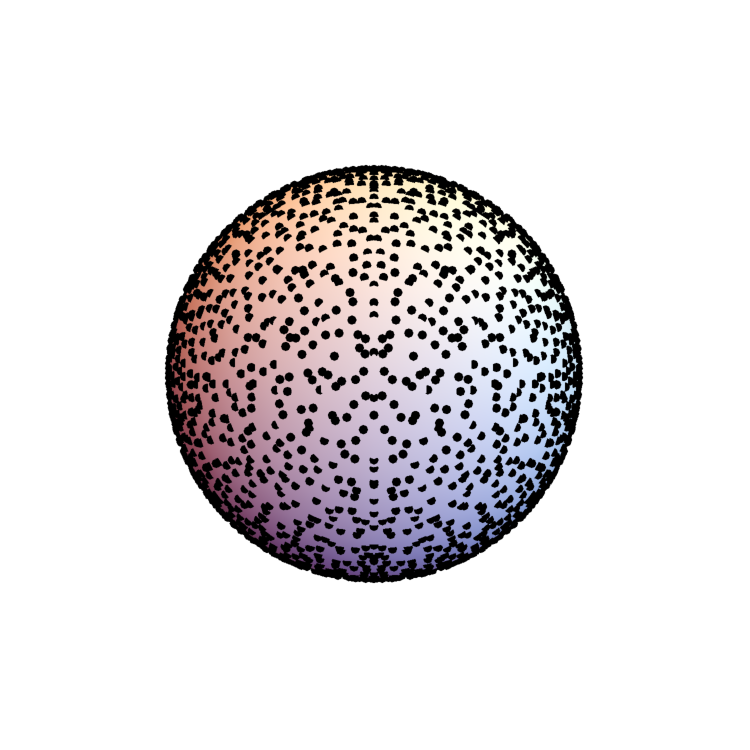
\includegraphics[width=2.5in]{det5000.pdf} 
   \caption{5000 determinantal points}
   \label{fig:example}
\end{figure}

}

\frame{
\frametitle{Spherical Cap Discrepancy}

\begin{figure}[htbp] %  figure placement: here, top, bottom, or page
   \centering
   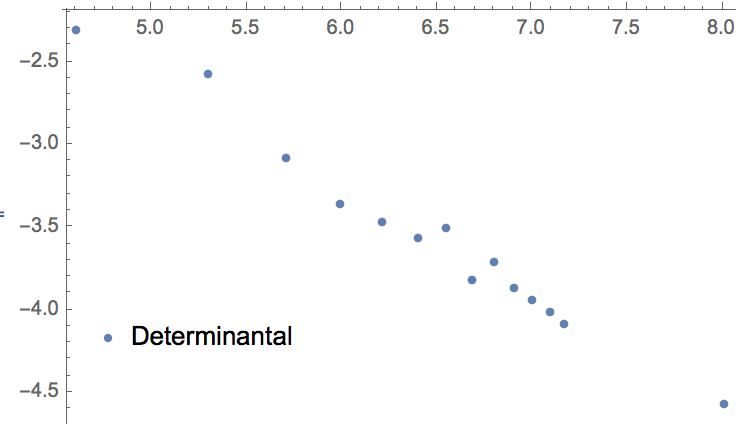
\includegraphics[width=3in]{detgraph.png} 
   \caption{$\log(N)$-$\log(D)$ plot for determinantal points}
   \label{fig:example}
\end{figure}

}


\frame{
\frametitle{Spherical Cap Discrepancy}
\begin{itemize}

\item It is know there exist good point sets $X_N$ on the sphere satisfying  $D(X_N)$ bounded by $O(N^{-3/4}\sqrt{\log N})$ and a lower bound for all points sets of $\Omega (N^{-3/4})$.  Constructions are probabilistic; we can check samples.
\vspace{1em}
\item Uniform random points are bounded by $O(N^{-1/2})$ (\emph{a.s.}). 
\vspace{1em}

\end{itemize}
}



\frame{
\frametitle{Spherical Cap Discrepancy}

\begin{figure}[htbp] %  figure placement: here, top, bottom, or page
   \centering
   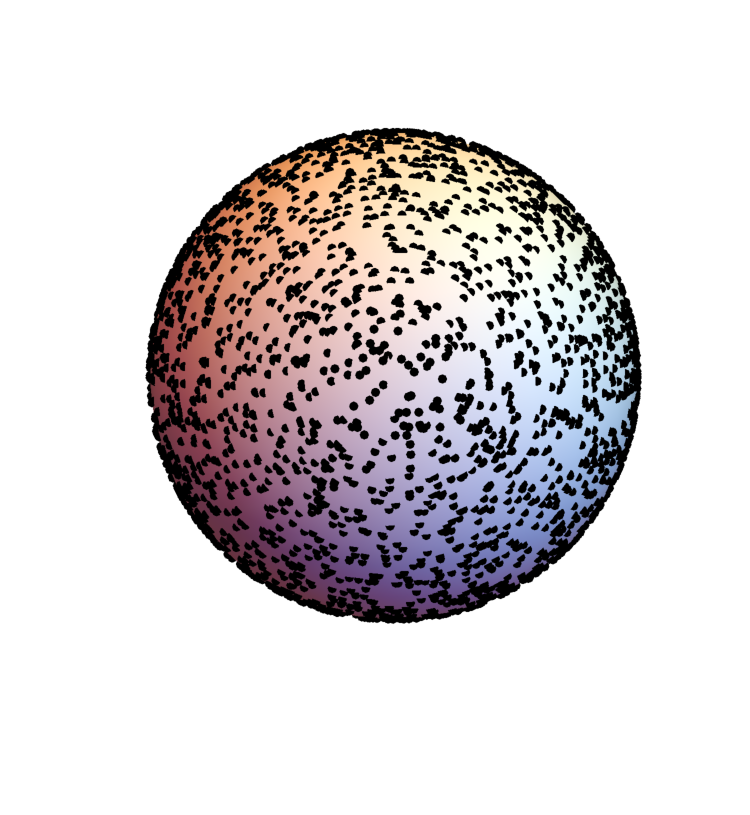
\includegraphics[width=2.5in]{uniform5000.pdf} 
   \caption{5000 psudo-random points}
   \label{fig:example}
\end{figure}

}

\frame{
\frametitle{Spherical Cap Discrepancy}

\begin{figure}[htbp] %  figure placement: here, top, bottom, or page
   \centering
   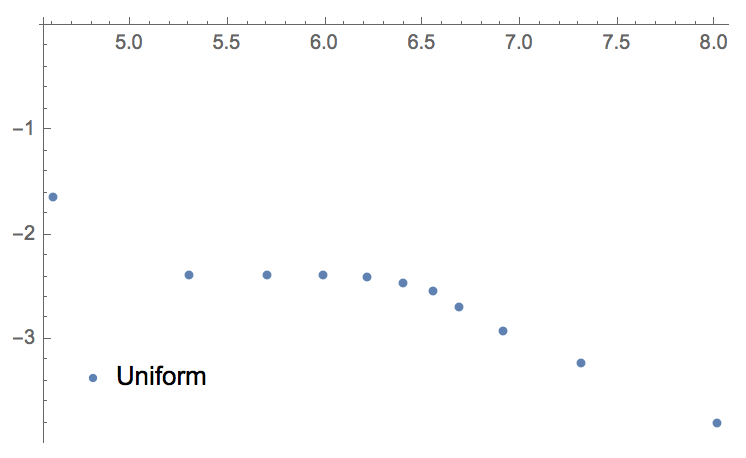
\includegraphics[width=3in]{uniformgraph.png} 
   \caption{$\log(N)$-$\log(D)$ plot for uniform random points}
   \label{fig:example}
\end{figure}

}


\frame{
\frametitle{Spherical Cap Discrepancy}
\begin{itemize}

\item It is know there exist good point sets $X_N$ on the sphere satisfying  $D[X_N]$ bounded by $O(N^{-3/4}\sqrt{\log N})$ and a lower bound for all points sets of $\Omega (N^{-3/4})$.  Constructions are probabilistic; we can check samples.
\vspace{1em}
\item Uniform random points are bounded by $O(N^{-1/2})$ (\emph{a.s.}). 
\vspace{1em}
\item It is conjectured that the Fibonacci points on the sphere have low discrepancy, perhaps optimal, but they are only known to be as good as random points.
\end{itemize}
}


\frame{
\frametitle{Spherical Cap Discrepancy}

\begin{figure}[htbp] %  figure placement: here, top, bottom, or page
   \centering
   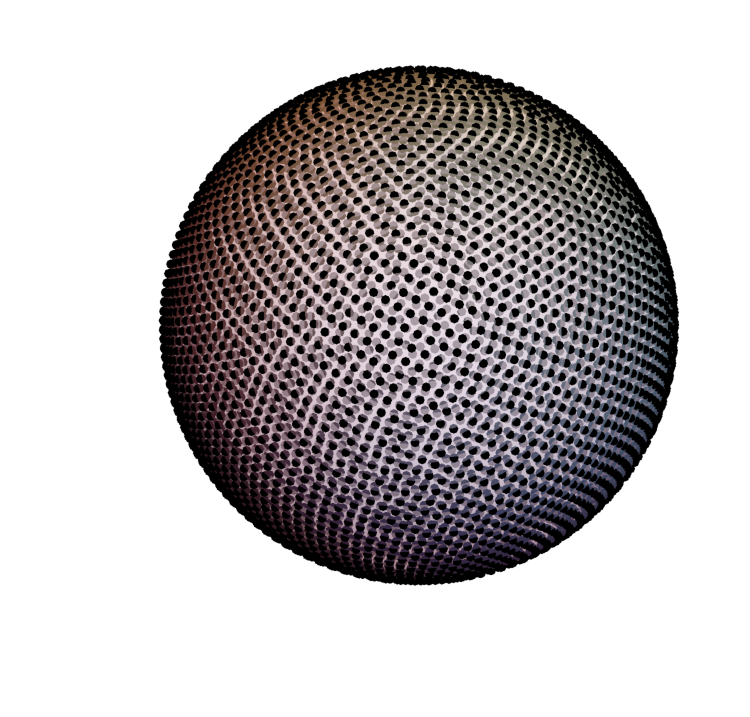
\includegraphics[width=2.5in]{fib5000.pdf} 
   \caption{5000 Fibonacci points}
   \label{fig:example}
\end{figure}

}

\frame{
\frametitle{Spherical Cap Discrepancy}

\begin{figure}[htbp] %  figure placement: here, top, bottom, or page
   \centering
   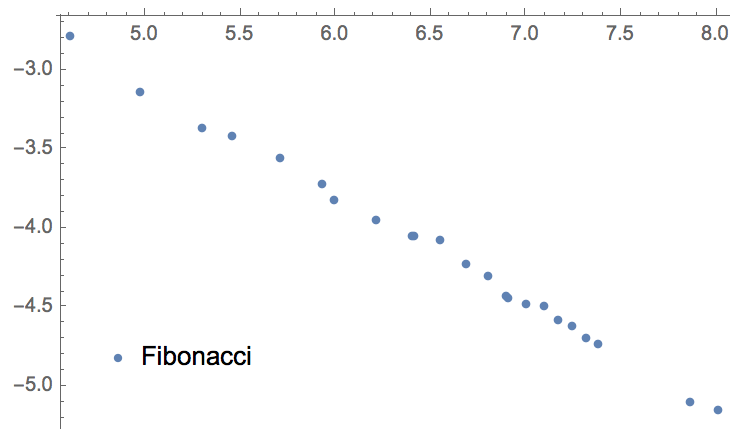
\includegraphics[width=3in]{fibgraph.png} 
   \caption{$\log(N)$-$\log(D)$ plot for Fibonacci points}
   \label{fig:example}
\end{figure}

}


\frame{
\frametitle{Spherical Cap Discrepancy}

Some other ``good" point sets.

\begin{itemize}
\item Lubotzky-Phillips-Sarnak points generated by irrational rotations.
\vspace{1em}
\item Spiral points other than the Fibonacci points.
 \vspace{1em}
\end{itemize}
}




\frame{
\frametitle{Spherical Cap Discrepancy}

\begin{figure}[htbp] %  figure placement: here, top, bottom, or page
   \centering
   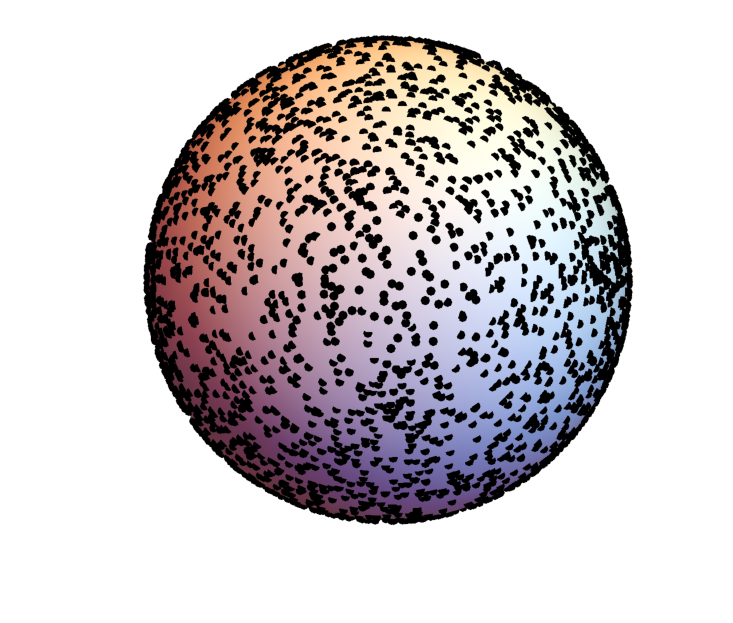
\includegraphics[width=2.5in]{lps5000.pdf} 
   \caption{5000 Lubotzky-Phillips-Sarnak points}
   \label{fig:example}
\end{figure}

}

\frame{
\frametitle{Spherical Cap Discrepancy}

\begin{figure}[htbp] %  figure placement: here, top, bottom, or page
   \centering
   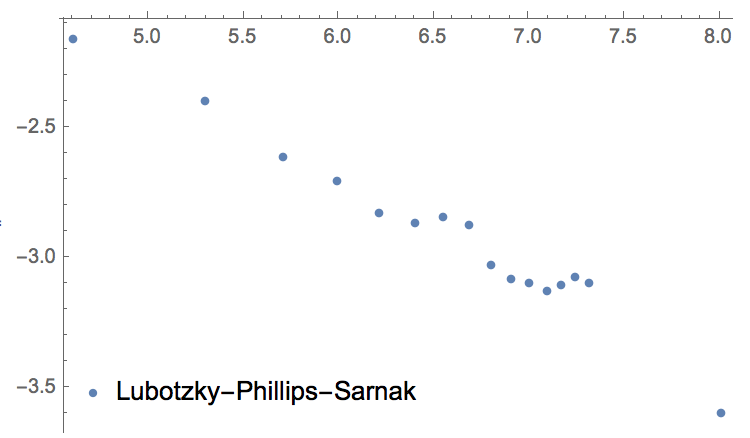
\includegraphics[width=3in]{lpsgraph.png} 
   \caption{$\log(N)$-$\log(D)$ plot for Lubotzky-Phillips-Sarnak points}
\end{figure}

}

\frame{
\frametitle{Spherical Cap Discrepancy}

\begin{figure}[htbp] %  figure placement: here, top, bottom, or page
   \centering
   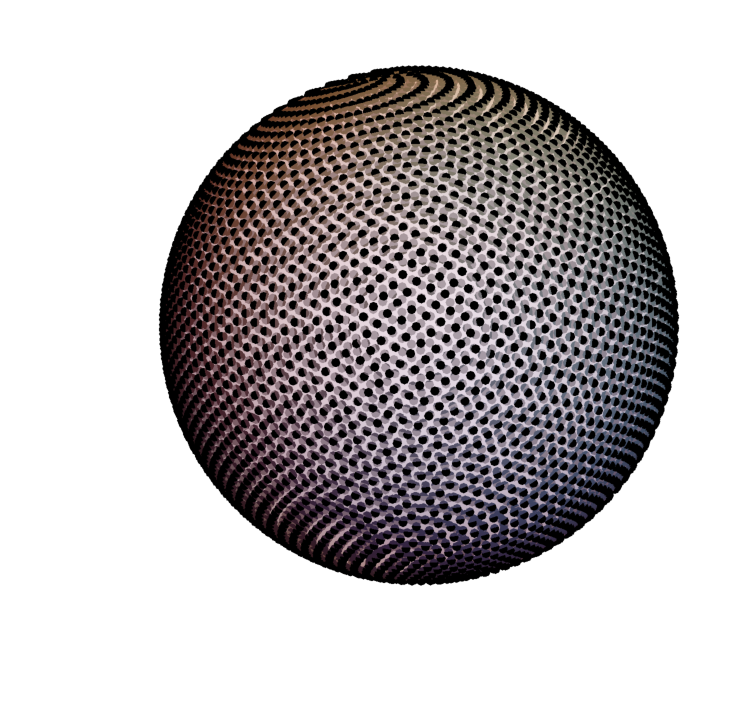
\includegraphics[width=2.5in]{e5000.pdf} 
   \caption{5000 spiral points}
\end{figure}

}

\frame{
\frametitle{Spherical Cap Discrepancy}

\begin{figure}[htbp] %  figure placement: here, top, bottom, or page
   \centering
   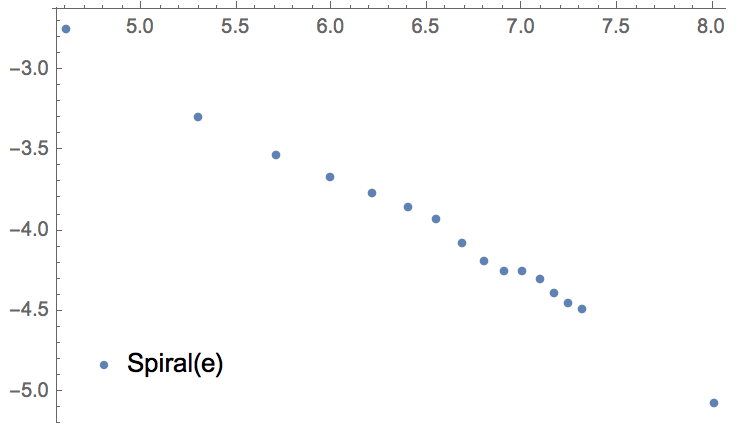
\includegraphics[width=3in]{egraph.png} 
   \caption{$\log(N)$-$\log(D)$ plot for spiral points}
\end{figure}

}



\frame{
\frametitle{Spherical Cap Discrepancy}

\begin{figure}[htbp] %  figure placement: here, top, bottom, or page
   \centering
 \hspace{.8em} 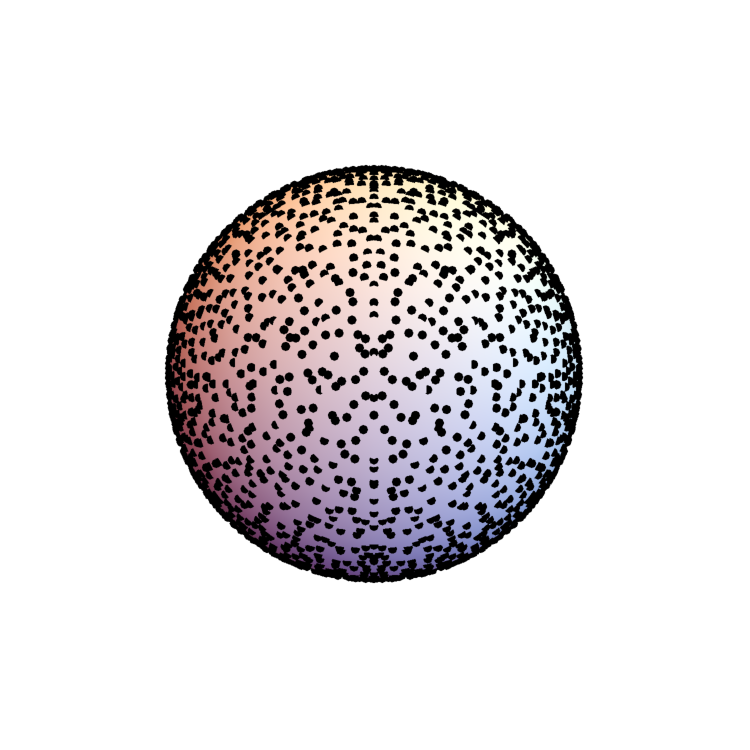
\includegraphics[width=1in]{det5000.pdf} \hspace{1em}
      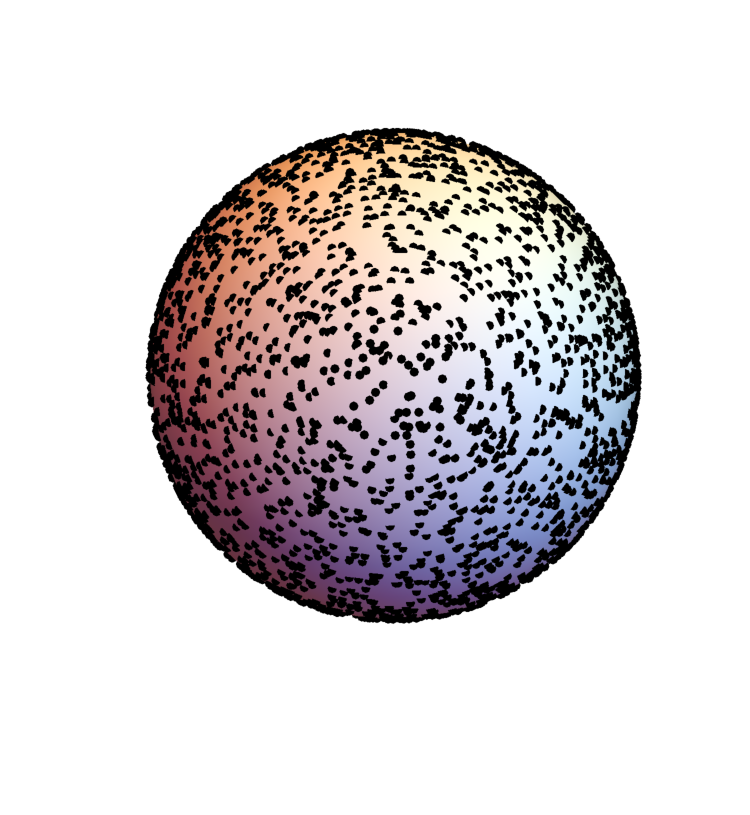
\includegraphics[width=1in]{uniform5000.pdf} \hspace{1em}
         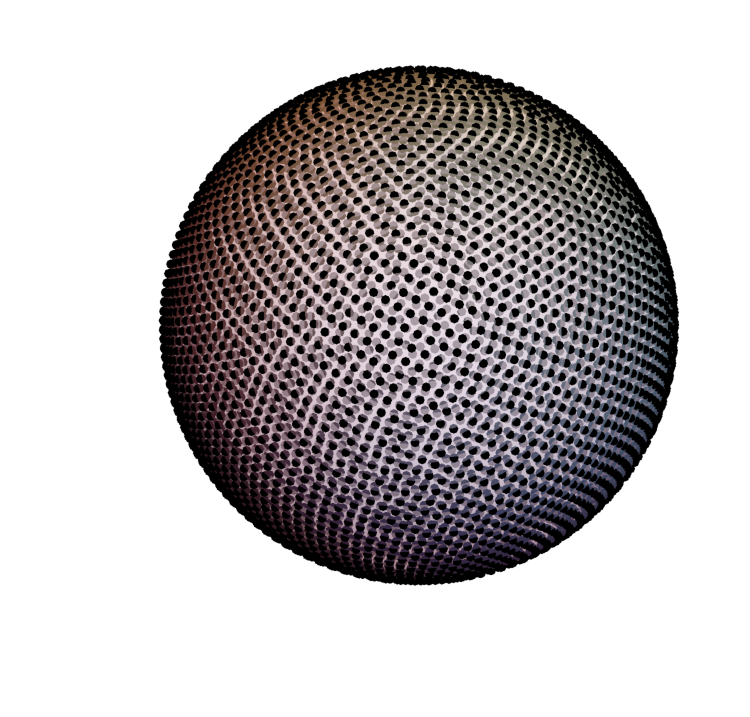
\includegraphics[width=1in]{fib5000.pdf} \newline
          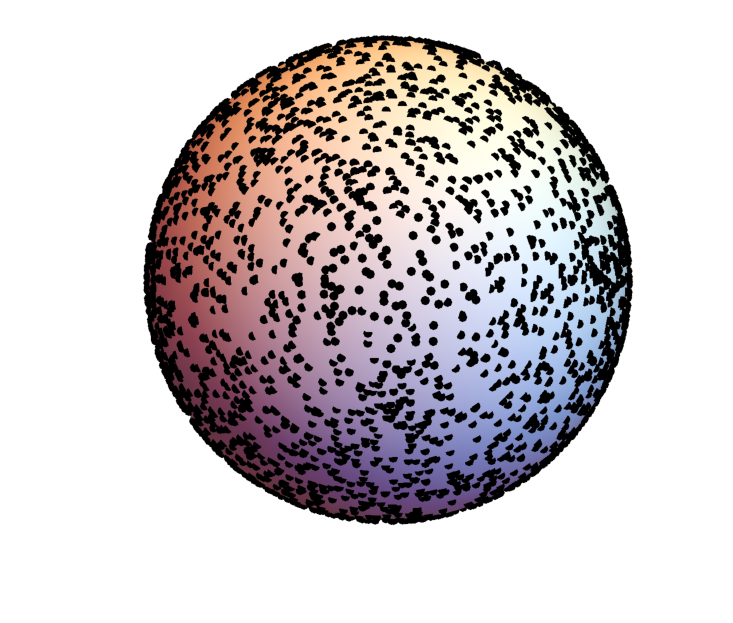
\includegraphics[width=1in]{lps5000.pdf} \hspace{1em}
               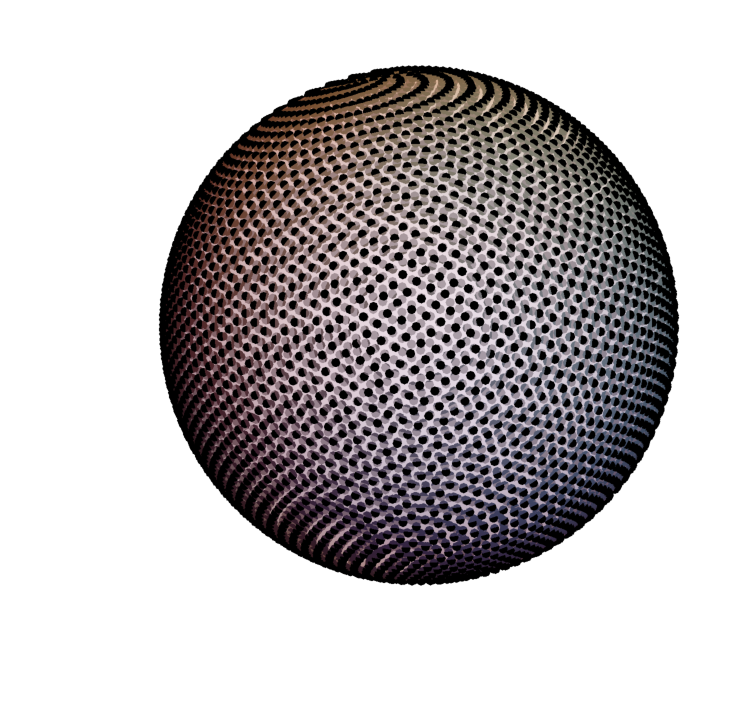
\includegraphics[width=1in]{e5000.pdf} 

   \label{fig:example}
\end{figure}

}



\frame{
\frametitle{Spherical Cap Discrepancy}

\begin{figure}[htbp] %  figure placement: here, top, bottom, or page
   \centering
   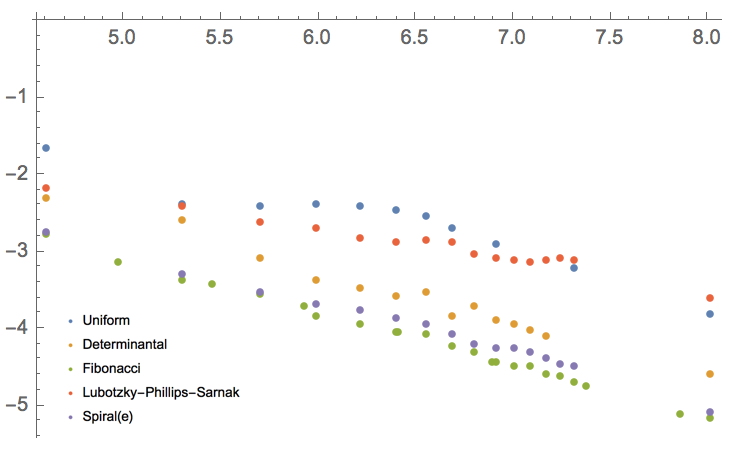
\includegraphics[width=3in]{pointplot.png} 
   \caption{$\log(N)$-$\log(D)$ plot combined}
\end{figure}
}



\frame{
\frametitle{Computation}
\begin{itemize}
\item Computing the $L^2$-discrepancy of a set of points can be done via \textbf{Stolarsky's Invariance Principle}, which states 
		\[
		\frac{1}{n^2} \sum_{i\ne j} \|x_i-x_j\| + K_d\, D_{L^2}^2[X_n] = \iint \| x-y\| \,\mathrm{d}\sigma(x)\mathrm{d}\sigma(y),
		\]
	where $K_d$ is a known constant depending only on the dimension $d$.
	
\item Based on results for discrepancy in boxes, it is likely that computing the spherical cap discrepancy is NP-hard. 
		
\end{itemize}
\vspace{1em}
\begin{remark}
There is still a nice algorithm for computing the discrepancy.
 \end{remark}

}

\frame{

\frametitle{Computation}
In the case of the star discrepancy, an algorithm was described by Niederreiter that exactly computes the star discrepancy.

\begin{itemize}
\item Note that the discrepancy function achieves local extrema when the measuring sets are ``captured."

\item This is a finite set, so enumerate and take the maximum.
\end{itemize}

A similar approach works for spherical caps.  It is a brute force approach that is exponential in dimension, but it is polynomial in the number of points.  To ``capture" a cap on $\mathbb{S}^d$ requires $d+1$ points or fewer, and $\binom{N}{d+1}$ is $O(N^{d+1})$.  \vspace{1em}

Comparing points gives an extra factor of $N$, so the runtime is $O(N^{d+2}).$  There are possible improvements with clever sorting, at some cost in memory.


}


\frame{

\frametitle{Computation}

\begin{figure}[htbp] %  figure placement: here, top, bottom, or page
   \centering
   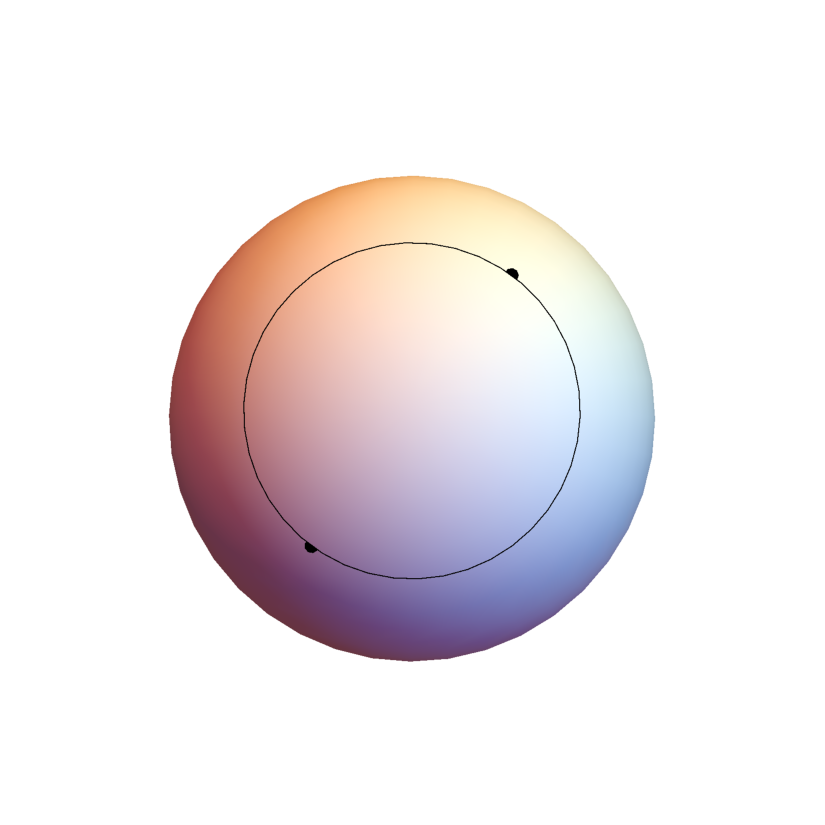
\includegraphics[scale=.4]{twopoints.pdf} 
    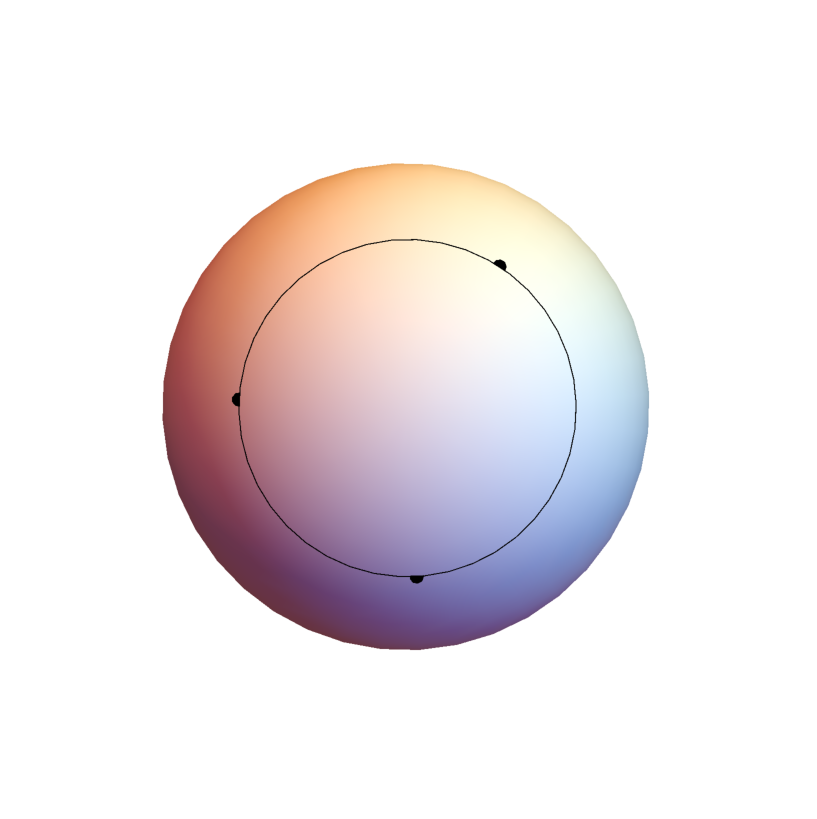
\includegraphics[scale=.4]{threepoints.pdf} 
   \label{fig:example}
\end{figure}



}




\frame{
\frametitle{Computation}
\begin{itemize}
\item This algorithm illustrates some of the issues with large constants in polynomial time algorithms, and with the implementation.  Just optimizing the code for the brute force algorithm can the time for several thousand points from several hundred years to a few hours.  
\vspace{1em}
\item Ways to increase speed: Sort with respect to a known good set using the triangle inequality.  Use a sweep pivoting on $d$ points.  These both cost memory.
\vspace{1em}
\item It is also a massively parallel problem.  In principle, we can compute discrepancy for millions of points relatively quickly.  
\end{itemize}
%\begin{remark}
%This is the experimental part of this project:  Implement and optimize our code and build a database of discrepancies for interesting point sets. 
%\end{remark}


}

\frame{
\frametitle{Optimization}

This algorithm hints at some optimization methods, but it really seems to depends on the labeled partitioning of $N$.  For a simplex, it works out nicely.  
\vspace{1em}

Four points on $\mathbb{S}^2$ can almost be optimized by hand.  For a lower bound, consider that discrepancy is a max-type function and symmetric across a cap $C$, which allows one to pass supporting points across the boundary of a cap to find stationary points.

\vspace{1em}
This gives an easy system to solve, where the important part is:
\[
|\textrm{Vol}(C) - 1/4| = |1-\textrm{Vol}(C)|\implies  \textrm{Vol}(C)=5/8, \, D[X_N]>3/8.
\]
\begin{remark}
This does not hold for the regular simplex.  
\end{remark}
}



\frame{
\frametitle{Optimization}

\begin{figure}[htbp] %  figure placement: here, top, bottom, or page
   \centering
   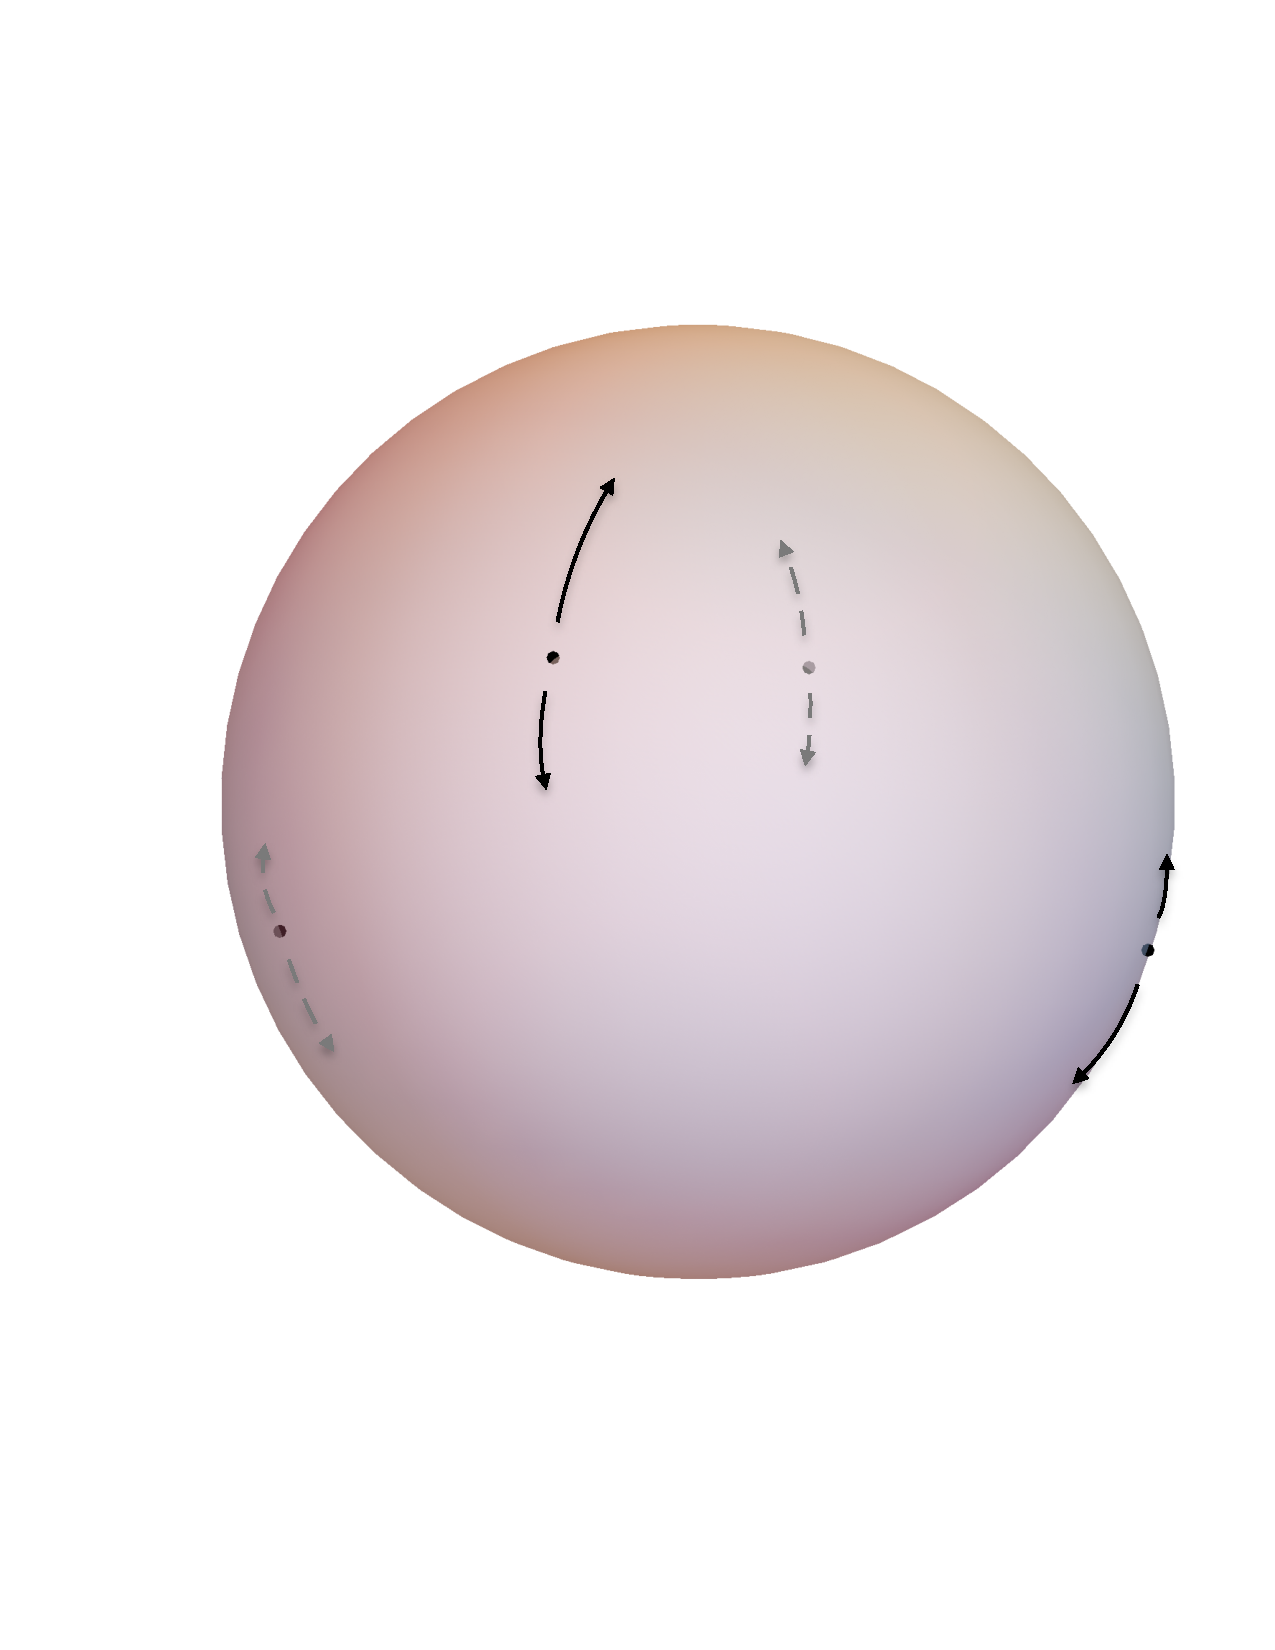
\includegraphics[scale=.3]{fourpoint2.pdf} 
   \caption{A very simple family of four points.}
   \label{fig:example}
\end{figure}

}

\frame{
\frametitle{Optimization}

We can symbolically solve to give 3-point discrepancies of 

\[
\frac{512+19 \sqrt{466-38 \sqrt{105}}+\sqrt{210
   \left(233-19 \sqrt{105}\right)}}{2048}
\]

\[
\frac{1024-19 \sqrt{466-38 \sqrt{105}}-\sqrt{210
\left(233-19 \sqrt{105}\right)}}{2048}
\]
\centering

\vspace{1cm}
(which also happen to be 3/8!)

}

\frame{
\frametitle{Optimization}

\begin{figure}[htbp] %  figure placement: here, top, bottom, or page
   \centering
   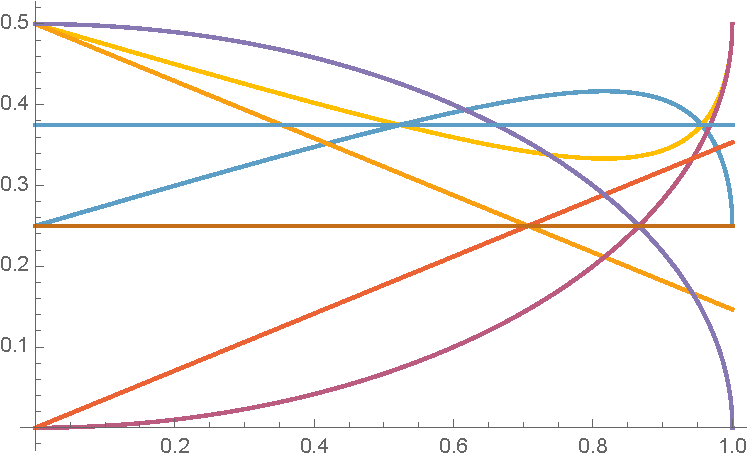
\includegraphics[scale=.7]{pointplot.pdf} 
   \caption{3-point and 2-point discrepancies for the tetrahedral family}
   \label{fig:example}
\end{figure}

}

\frame{
\frametitle{Optimization}

\begin{figure}[htbp] %  figure placement: here, top, bottom, or page
   \centering
   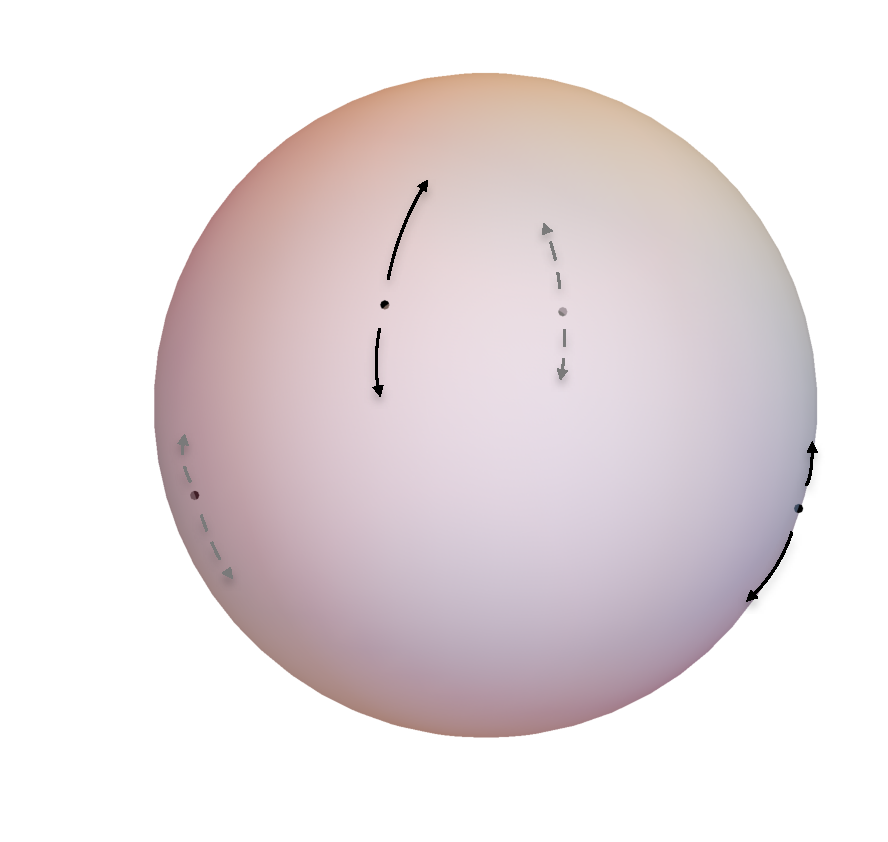
\includegraphics[scale=.5]{fourpoint.pdf} 
   \caption{A minimal discrepancy set}
   \label{fig:example}
\end{figure}


}


%\frame{
%\frametitle{\,}
%\begin{figure}[htbp] %  figure placement: here, top, bottom, or page
%   \centering
%   
\includegraphics[scale=.8]{thanks.png} 
%   \caption{}
%   \label{fig:example}
%\end{figure}
%}


\end{document}

